\documentclass{beamer}
\usetheme{ConnectivityLab}
\usepackage{times}
\usepackage{graphicx}
\usepackage{verbatim}
\usepackage{outlines}
\usepackage{fancyhdr}
\usepackage{subfigure}
\usepackage{cancel}
\usepackage{bibentry}
\usepackage{varwidth}
\usepackage{etoolbox}
\usepackage{epstopdf}

%%%%%%%%%%%%%%%%%%%%%%%%%%%%%%%%%%%%%%%%%%%%%%%%%%%%%%
%%%%%%%%%%%%%%%%%%%%%%%%%%%%%%%%%%%%%%%%%%%%%%%%%%%%%%

\title {
    Retransmission-based Access Class Barring for RAN overload control in Machine Type Communications
}
\author {
    Yin-Hong, Hsu
}
\date {
    09 22, 2016
}

%%%%%%%%%%%%%%%%%%%%%%%%%%%%%%%%%%%%%%%%%%%%%%%%%%%%%%
%%%%%%%%%%%%%%%%%%%%%%%%%%%%%%%%%%%%%%%%%%%%%%%%%%%%%%

\begin{document}
\begin{frame}
    \titlepage
\end{frame}

%%%%%%%%%%%%%%%%%%%%%%%%%%%%%%%%%%%%%%%%%%%%%%%%%%%%%%
%%%%%%%%%%%%%%%%%%%%%%%%%%%%%%%%%%%%%%%%%%%%%%%%%%%%%%

\begin{frame}{Outline}
    \tableofcontentsgather
    \tableofcontents
\end{frame}

%%%%%%%%%%%%%%%%%%%%%%%%%%%%%%%%%%%%%%%%%%%%%%%%%%%%%%
%%%%%%%%%%%%%%%%%%%%%%%%%%%%%%%%%%%%%%%%%%%%%%%%%%%%%%
\section{Aim}

%%%%%%%%%%%%%%%%%%%%%%%%%%%%%%%%%%%%%%%%%%%%%%%%%%%%%%
%%%%%%%%%%%%%%%%%%%%%%%%%%%%%%%%%%%%%%%%%%%%%%%%%%%%%%
\begin{frame}{Aim} 
    \begin{itemize}
        \item \textbf{In order to alleviate the RAN overload,}
    \end{itemize}

    \begin{itemize}
        \item \textbf{we focus on the objective that can increase access success probability and relieve the access delays.}
    \end{itemize}
\end{frame}

%%%%%%%%%%%%%%%%%%%%%%%%%%%%%%%%%%%%%%%%%%%%%%%%%%%%%%
%%%%%%%%%%%%%%%%%%%%%%%%%%%%%%%%%%%%%%%%%%%%%%%%%%%%%%
\section{Solution}

\begin{frame}{Solution}
    \begin{figure}[t]
        \centering
        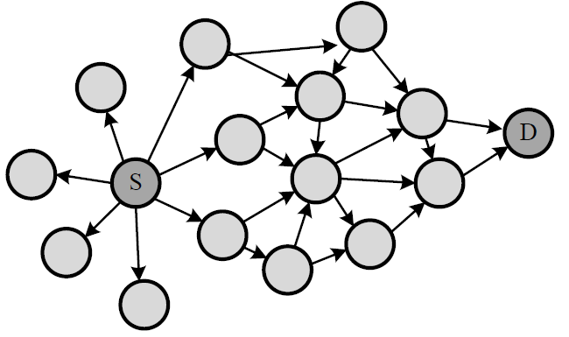
\includegraphics[width=0.6\textwidth]{figures/Fig_1-1.png}
        \setbeamerfont{caption}{size=\tiny}
        \caption{Some Figure Description}
    \end{figure}
\end{frame}

%%%%%%%%%%%%%%%%%%%%%%%%%%%%%%%%%%%%%%%%%%%%%%%%%%%%%%
%%%%%%%%%%%%%%%%%%%%%%%%%%%%%%%%%%%%%%%%%%%%%%%%%%%%%%
\section{Result}

%%%%%%%%%%%%%%%%%%%%%%%%%%%%%%%%%%%%%%%%%%%%%%%%%%%%%%
%%%%%%%%%%%%%%%%%%%%%%%%%%%%%%%%%%%%%%%%%%%%%%%%%%%%%%
\begin{frame}{Result}
    \begin{center}
        \begin{tabular}{ | l | l | }
            \hline
                Parameter                                   &       Value               \\ \hline
                Simulation Count                            &       100 thousand        \\ \hline
                Area Width / Length                         &       40.0 meter          \\ \hline
                eNB Intensity ($\lambda_{B}$)               &       0.01 $m^{-2}$       \\ \hline
                CeUE Intensity ($\lambda_{C}$)              &       0.15 $m^{-2}$       \\ \hline
                DeUE Intensity ($\lambda_{D}$)              &       0.15 $m^{-2}$       \\ \hline
                Path Loss Exponent ($\alpha$)               &       4.0                 \\ \hline
                eNB Power ($P_{B}$)                         &       43.0 dBm            \\ \hline
                Maximum Medium Access Prob. $\tilde{p}$     &       0.9                 \\
            \hline
        \end{tabular}
    \end{center}
\end{frame}

\end{document}
